% Created 2020-11-27 Fri 11:04
% Intended LaTeX compiler: pdflatex
\documentclass[11pt]{article}
\usepackage[utf8]{inputenc}
\usepackage[T1]{fontenc}
\usepackage{graphicx}
\usepackage{grffile}
\usepackage{longtable}
\usepackage{wrapfig}
\usepackage{rotating}
\usepackage[normalem]{ulem}
\usepackage{amsmath}
\usepackage{textcomp}
\usepackage{amssymb}
\usepackage{capt-of}
\usepackage{hyperref}
\documentclass{article}
\usepackage{here}
\usepackage{xcolor}
\usepackage[margin=3.0cm]{geometry}
\usepackage{amsmath}
\usepackage{parskip}
\renewcommand\arraystretch{1.4}
\documentclass[12pt]{report}
\author{Fatih Kaan Salgır - 171044009}
\date{}
\title{CSE 331 Computer Organizations Homework 2}
\hypersetup{
 pdfauthor={Fatih Kaan Salgır - 171044009},
 pdftitle={CSE 331 Computer Organizations Homework 2},
 pdfkeywords={},
 pdfsubject={},
 pdfcreator={Emacs 27.1 (Org mode 9.3.7)}, 
 pdflang={English}}
\begin{document}

\maketitle


\section{Algorithm Explanation}
\label{sec:orga1306c2}

\textbf{Inputs:} Array of elements along with its size and number to be checked  

\textbf{Output:} 1 if if sub elements of the array can sum up to this number, 0 otherwise.

If there are elements in the array can sum up to the number; an element can either be inclueded or excluded to this group. Therefore elements need to be checked until find a solution or there are no elements left. For any element there are 2 possibilities, inclueded or excluded.

Without optimization algorithm looks like;

\noindent\rule{\textwidth}{0.5pt}
\begin{verbatim}
1. Check rest of the array without the element.
2. Check rest of the array with the element.

- Return 1 if summed values are equal to target number.
- Return 0 if size exceed.
\end{verbatim}

\noindent\rule{\textwidth}{0.5pt}

I have preferd to decrase the number, and check if it is 0. Instead of summing up.


\subsection{Optimzations}
\label{sec:orgf03a81d}
\begin{itemize}
\item If summed number exceed to target number, it is pointless to keep adding. (In my case \texttt{num < 0})
\item If element is equal to target or remaining value is equal the target then return 1.
\end{itemize}


I impemented the printing numbers in assembly. I did not store them in a structure, only print the screen when it is found.

\textbf{Note:} Results might not be the same with the pdf, but they are accurate. So, it might be slower or faster according to input data.

\newpage

\section{Test Cases}
\label{sec:orgee3402c}

C++ code output:

\begin{center}
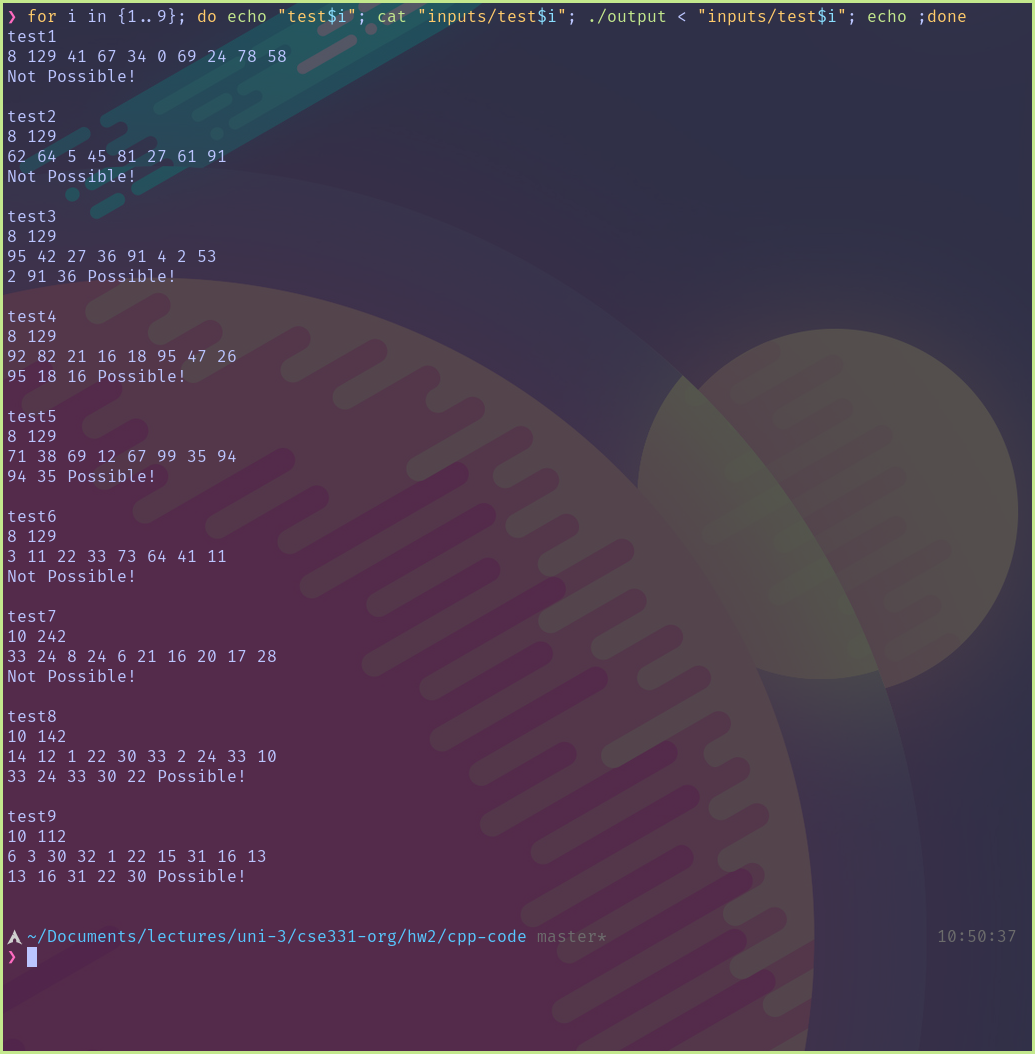
\includegraphics[width=460px]{Test_Cases/2020-11-27_10-52-36_screenshot.png}
\end{center}


\newpage

MARS output:

\begin{center}
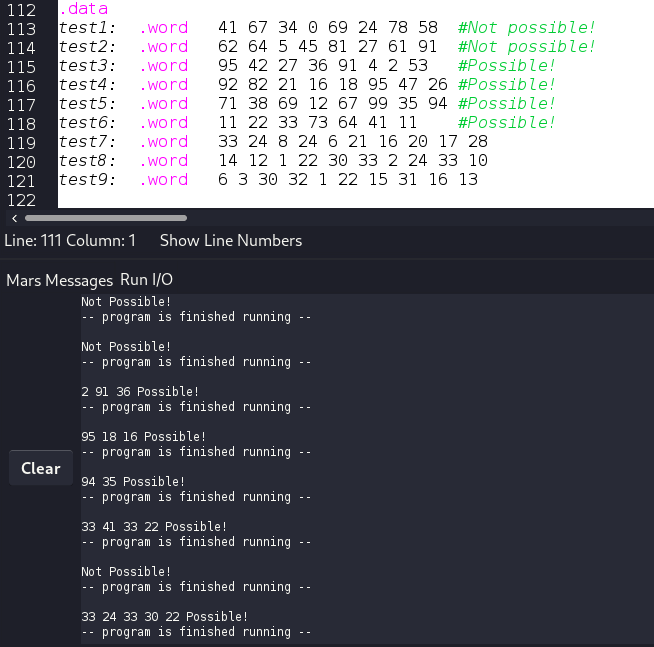
\includegraphics[width=400px]{Test_Cases/2020-11-27_11-03-36_screenshot.png}
\end{center}
\end{document}